\chapter{Самоиндукция и взаимная индукция}

\section{Индуктивность контура}

    Рассмотрим контур \( C \) с током \( i \). Ток \( i \) создаёт магнитное
    поле \( \vec{B} \). Следовательно, через контур есть магнитный поток 
    \[ 
        \Phi = \iint\limits_S \vec{B}\cdot\dd \vec{S}.
    \]
    Поле \( \vec{B} \), согласно закону Био-Савара, пропорционально току
    \( i \), следовательно, поток \( \Phi \) так же пропорционален току \( i \).
    
    Эту зависимость можно записать так:
    \begin{equation}
        \Phi = Li
        \label{eq12:1}
    \end{equation}
    
    \begin{definition}
        Коэффициент пропорциональности \( L \) между током \( i \) в контуре и
        созданном им магнитным потоком \( \Phi \) через контур в (\ref{eq12:1})
        называется \textbf{индуктивностью}.
    
        Таким образом, по определению:
        \[
            L = \frac{\Phi}{i}.
        \]
    \end{definition}
    \begin{figure}[!b]
        \center
        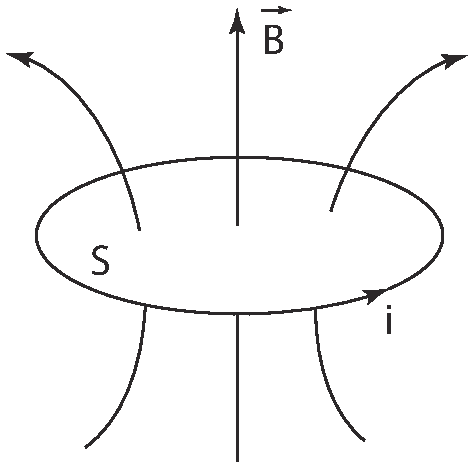
\includegraphics[width=0.3\textwidth]{lec12/inductance.pdf}
        \caption{Индуктивность -- характеристика контура, определяемая лишь его
            геометрией}
    \end{figure}    
    Индуктивность \( L \) зависит только от геометрии контура и от среды, в
    которую он помещён, и не зависит от тока.
    
    \begin{remark}
        При определении индуктивности по формуле (\ref{eq12:1}) провод контура
        не должен быть слишком толстым, ибо для толстых проводов не определены
        понятия площади контура \( S \) и, следовательно, потока \( \Phi \).
        Однако, провод не должен быть и бесконечно тонким, так как при
        \( r_{\textit{пров}} \to 0 \) поле \( B \sim r^{-1} \to \infty \) и его
        поток
        \[
            \Phi = \iint\limits_S \vec{B}\cdot\dd \vec{S} \to \infty.
        \]
        В этом смысле определение (\ref{eq12:1}) некорректно.
    \end{remark}
    
    \begin{example}
        Вычислить индуктивность соленоида (\( N, S, l \)).
    \end{example}
    \begin{solution}
        Поле в соленоиде: \( B = \mu_0 \frac{N}{l}i \) -- однородно. Поток 
        \( \Phi \) через \( N \) витков:
        \[
            \Phi = \iint_S \vec{B}\cdot\dd \vec{S} = (BS)N =
            \mu_0 \frac{N^2}{l}Si.
        \]
        По определению (\ref{eq12:1}):
        \[
            L = \frac{\Phi}{i} = \mu_0 \frac{N^2}{l}S.
        \]
    \end{solution}
    
    \begin{example}
        Вычислить погонную индуктивность \( L_0 = \frac{L}{l} \) коаксиальной
        линии (\( R_1, R_2, \mu = 1 \)).
    \end{example}
    \begin{solution}
        Поле в коаксиальной линии (\( R_1 < r < R_2 \))
        \[
            B = \frac{\mu_0 i}{2\pi r}.
        \]
        Вычислим поток \( \Phi \) этого поля через продольное сечение зазора
        (\( R_1 < r < R_2 \)). Сначала вычислим поток \( \dd \Phi \) через
        полоску \( \dd  S = l\dd  r \):
        \[
            \dd \Phi = B(r)\dd  S = \frac{\mu_0 i}{2\pi r}l\dd  r.
        \]
        Тогда поток через всё сечение:
        \[
            \Phi = \int\limits_{R_1}^{R_2} \frac{\mu_0 i}{2\pi r}l\dd  r = 
            \frac{\mu_0 i}{2\pi}l \int\limits_{R_1}^{R_2} \frac{\dd  r}{r} =
            \frac{\mu_0 il}{2\pi}\ln\frac{R_1}{R_2}.
        \]
        Индуктивность по (\ref{eq12:1}):
        \[
            L = \frac{\mu_0 il}{2\pi}\ln\frac{R_1}{R_2}\cdot\frac{1}{i} =
            \frac{\mu_0 l}{2\pi}\ln\frac{R_1}{R_2}.
        \]
        Тогда погонная индуктивность
        \[
            L_0 = \frac{L}{l} = \frac{\mu_0}{2\pi}\ln\frac{R_1}{R_2}.
        \]
    \end{solution}

    \begin{figure}[b!]
        \center
        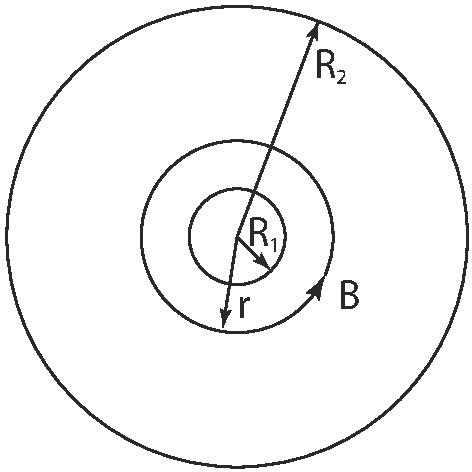
\includegraphics[width=0.3\textwidth]{lec12/coaxial_line.pdf}
        \caption{Коаксиальная линия. Торец}
    \end{figure}    

\section{Самоиндукция}

    Рассмотрим проводящий контур. Будем наращивать ток \( i \) в нём.
    Следовательно, будет увеличиваться поле \( \vec{B} \) и его поток \( \Phi \).
    Согласно закону ЭМИ, в контуре наведется ЭДС:
    \[
        \EDS = -\frac{\dd \Phi}{\dd  t} = \EDS_{\textit{си}}.
    \]
    А так как \( \Phi = Li \), то
    \begin{equation}
        \EDS_{\textit{си}} = -L\frac{\dd  i}{\dd  t}.
        \label{eq12:2}
    \end{equation}
    
    \begin{definition}
        Явление появления в контуре ЭДС при изменении тока в нём называется
        \textbf{самоиндукцией}, а само ЭДС -- \textbf{ЭДС самоиндукции}
        \( \EDS_{\textit{си}} \). Это ЭДС направлено против изменения тока.
    \end{definition}
    
\section{Определения и размерности магнитных величин}

    \begin{enumerate}
    \item Индуктивность в СИ: \textbf{Гн} -- Генри:
        \( L = 1 \)Гн -- индуктивность такого контура, в котором наводится ЭДС 
        \( \EDS_{\textit{си}} = 1 \)В при скорости изменения тока в
        \( 1 \text{А}/\text{с} \).
        \[
            [L] = \left[\frac{\EDS}{\frac{\dd  i}{\dd  t}}\right] = 
            \frac{\text{В}\cdot\text{с}}{\text{А}} = \text{Гн};
        \]
        
    \item Магнитный поток в СИ: \textbf{Вб} -- Вебер:
        \( \Phi = 1 \)Вб -- поток через контур с индуктивностью \( L = 1\)Гн при
        токе в нём \( i = 1\)А.
        \[
            [\Phi] = \left[Li\right] = \text{Гн}\cdot\text{А} = \text{Вб};
        \]
        
    \item Магнитное поле в СИ: \textbf{Тл} -- Тесла:
        \( B = 1 \)Тл -- однородное поле, создающее поток \( \Phi = 1\)Вб через
        площадку \( S = 1 \text{м}^2 \).
        \[
            [B] = \left[\frac{\Phi}{S}\right] = \frac{\text{Вб}}{\text{м}^2} =
            \text{Тл}.
        \]
    \end{enumerate}
    
\section{Энергия контура с током}
    Рассмотрим контур, в котором наращивается ток \( i \). Следовательно,
    появится ЭДС самоиндукции:
    \[
        \EDS_{\textit{си}} = -L\frac{\dd i}{\dd t}.
    \]
    Работа внешних сил (генератора) по перемещению заряда \( \dd  q \) против 
    \( \EDS_{\textit{си}} \) по определению
    \[
        \dd A = -\EDS_{\textit{си}}\dd q = L\frac{\dd i}{\dd t}\dd q = Li\dd i.
    \]
    А так как контур -- идеально проводящий, то тепловых потерь нет, и,
    следовательно, работа численно равна энергии, накопленной в контуре:
    \[
        A = W = \int\limits_0^i Li\dd  i = \frac{L i^2}{2}.
    \]
    Таким образом, энергия:
    \begin{equation}
        W = \frac{Li^2}{2}.
        \label{eq12:3}
    \end{equation}
    
\section{Распределение энергии в магнитном поле}
    Рассмотрим соленоид с током \( i \). Его индуктивность
    \[
        L = \mu_0 \frac{N^2}{l}S,
    \]
    а энергия, заключённая в нём
    \[
        W = \frac{Li^2}{2} = \frac{\mu_0 N^2 S}{2l}i^2 = 
        \frac{1}{2\mu_0} \left(\underbrace{\mu_0 \frac{N}{l} i}_{B}\right)^2
        \underbrace{lS}_{V_{\textit{сол}}} = \frac{B^2}{2\mu_0}V_{\textit{сол}}.
    \]
    А так как вне соленоида поля \( \vec{B} \) нет, то
    \( V_\textit{сол} = V_B \). Таким образом, \( W \sim V_B \). Можно сделать
    предположение о локализации энергии в поле \( \vec{B} \). Тогда
    \[
        w_B = \frac{W}{V_B} = \frac{B^2}{2\mu_0}
    \]
    объемная плотность энергии магнитного поля.
    
    Предположение оказывается правдой: если энергию токовой системы вычислять
    как энергию её поля
    \[
        W = \iiint\limits_{V_B} \frac{B^2}{2\mu_0} \dd  V,
    \]
    то результат всегда будет верным.
    
    \begin{remark}
        Из формулы (\ref{eq12:3}) получается корректное определение
        индуктивности:
        \begin{equation}
            L = 2\frac{W}{i^2},
        \end{equation}
        где \[ W = \iiint\limits_{V_B} \frac{B^2}{2\mu_0} \dd  V. \]
    \end{remark}
    
\section{Взаимная индукция}
    Рассмотрим два контура: \( C_1 \) и \( C_2 \). Пусть по контуру \( C_1 \)
    идет ток \( i_1 \). Тогда часть линий поля \( \vec{B}_1 \) пройдет через
    контур \( C_2 \). Тогда поток поля \( \vec{B}_1 \) через контур \( C_2 \)
    \begin{equation}
        \Phi_2 \sim i_1 \  \Rightarrow \  \Phi_2 = L_{21}i_1.
        \label{eq12:n1}
    \end{equation}

    \begin{figure}[b!]
        \center
        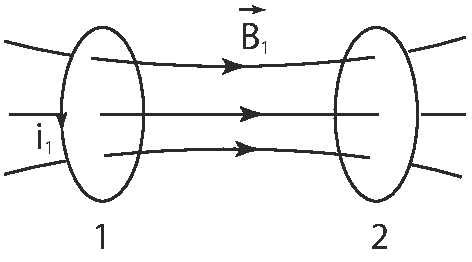
\includegraphics[width=0.3\textwidth]{lec12/mutual_inductance.pdf}
        \caption{Взаимная индукция}
    \end{figure}

    Аналогично, если создать ток \( i_2 \) на контуре \( C_2 \), то поток поля 
    \( \vec{B}_2 \) через \( C_1 \):
    \begin{equation}
        \Phi_1 = L_{12}i_2.
        \label{eq12:n2}
    \end{equation}
    
    \begin{definition}
        Коэффициенты \( L_{21} \) и \( L_{12} \) в формулах (\ref{eq12:n1}) и
        (\ref{eq12:n2}) называются \textbf{взаимными индуктивностями} двух
        контуров.
    \end{definition}
    
    Можно показать, что для любой пары контуров
    \[
        L_{21} = L_{12} \equiv M.
    \]
    Таким образом, \( \Phi_2 = Mi_1\) и \( \Phi_1 = Mi_2 \).
    
    \begin{definition}
        \textbf{Взаимная индуктивность пары контуров} \( M \) -- это парная
        характеристика двух токовых систем. Она зависит от геометрий систем и
        от среды, в которую они помещены.
    \end{definition}
    
    При изменении тока \( i_1 \) в контуре \( C_2 \) появляется ЭДС индукции:
    \begin{equation}
        \EDS_2 = -\frac{\dd \Phi_2}{\dd t} = -M\frac{\dd i_1}{\dd t}
        \label{eq12:n3}
    \end{equation}
    Аналогично, при изменении тока \( i_2 \) в контуре \( C_1 \) появляется ЭДС
    индукции:
    \[
        \EDS_1 = -\frac{\dd \Phi_1}{\dd t} = -M\frac{\dd i_2}{\dd t}.
    \]
    
    \begin{example}
        Вычислить взаимную индукцию пары коаксиальных соленоидов \( S_1 \) и
        \( S_2 \) одинаковой длины \( l \).
    \end{example}
    
    \begin{solution}
        Задаём ток в одном из соленоидов, например, \( i_2 \) в соленоиде
        \( S_2 \). Его поле
        \[
            B_2 = \mu_0 \frac{N_2}{l} i_2.
        \]
        Его поток через \( N_1 \) витков соленоида \( S_1 \):
        \[
            \Phi_1 = B_2 S_1N_1 = \mu_0 \frac{N_1N_2}{l} i_2S_1.
        \]
        Тогда взаимная индуктивность:
        \[
            M = \frac{\Phi_1}{i_2} = \frac{\mu_0 N_1N_2}{l}S_1.
        \]
    \end{solution}
    
    \begin{remark}
        Тот же результат получится, если задать ток \( i_1 \) в соленоиде
        \( S_1 \) и вычислить поток \( \Phi_2 \).
    \end{remark}
    
    \begin{example}
        Вычислить взаимную индукцию прямого длинного провода и прямоугольной рамки (\( a, b\)).
    \end{example}
    
    \begin{solution}
            Здесь \textit{удобно} задавать ток \( i \) в проводе и вычислять
            поток через рамку. Пусть в проводе задан ток \( i \). Тогда поле
            \[
                B = \frac{\mu_0 i}{2\pi r}.
            \]
            Поток через полоску \( S_{\textit{пол}} = b\dd  r \):
            \[
                \dd \Phi = B(r)b\dd  r = \frac{\mu_0 i}{2\pi r}b\dd  r,
            \]
            а весь поток:
            \[
                \Phi = \int\limits_l^{l + a} \frac{\mu_0 i}{2\pi r}b\dd  r =
                \frac{\mu_0 i}{2\pi}b \int\limits_l^{l + a} \frac{\dd  r}{r} =
                \frac{\mu_0 i}{2\pi}b\ln\left(1 + \frac{a}{l}\right). 
            \]
            По определению
            \[
                M = \frac{\Phi}{i} =
                \frac{\mu_0}{2\pi}b\ln\left(1 + \frac{a}{l}\right).
            \]
            При \( l \gg a \)
            \[
                M \approx \frac{\mu_0}{2\pi}b\frac{a}{l} = 
                \frac{\mu_0}{2\pi}\frac{S_{\textit{р}}}{l}.
            \]
            
            Если по проводу идет сигнал \( i = I\sin\omega t \), то в рамке
            будет ЭДС:
            \[
                \EDS_{\textit{р}} = M\frac{\dd i}{\dd t} =
                \underbrace{MI\omega}_{\EDS_A} \cos\omega t,
            \]
            \[
                \EDS_A = MI\omega = \frac{\mu_0 S_{\textit{р}}}{2\pi l}I\omega.
            \]
            Пусть \( I = 10 \)А, \( \omega = 1,6 \text{кГц} = 
            10^4 \text{рад}/\text{с} \), \( S_{\textit{р}} = 100 \text{см}^2 = 
            10^{-2} \text{м}^2 \), \( N_{\textit{р}} = 100 \)витков, 
            \( l = 10 \)м.
            
            Тогда амплитуда ЭДС:
            \[
                \EDS_A = \frac{\mu_0 S_{\textit{р}}}{2\pi l}I\omega = 
                2 \times 10^{-2} \text{мВ}.
            \] 
    \end{solution}
    
    \begin{figure}[!b]
        \center
        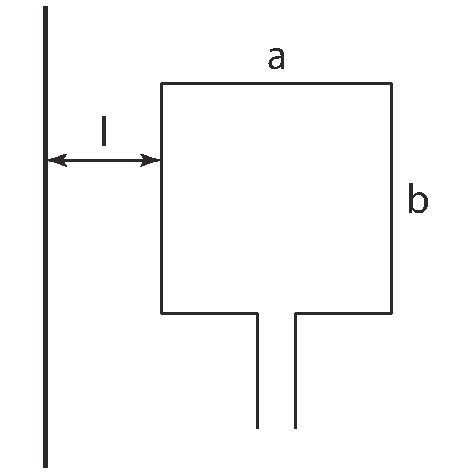
\includegraphics[width=0.3\textwidth]{lec12/wire_n_frame.pdf}
        \caption{Взаимная индукция рамки и провода}
    \end{figure}    

\section{Соединения катушек}
    
    Две катушки считаются \textit{магнитно-связанными}, если не слишком малая
    часть магнитного потока одной из них пронизывает витки другой.

    \begin{figure}[b!]
        \center
        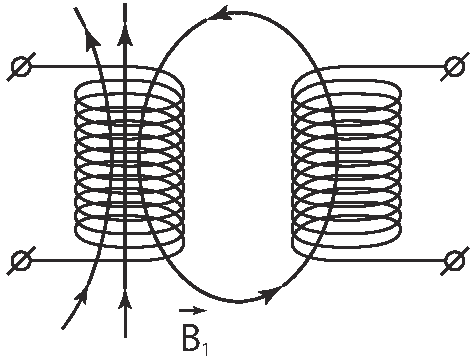
\includegraphics[width=0.3\textwidth]{lec12/coils_interaction.pdf}
        \caption{Магнитно-связанные катушки}
    \end{figure}
    
    Две катушки могут быть соединены как последовательно, так и параллельно.
    
    \subsection{Последовательное соединение}
    
    \begin{figure}[b!]
        \center
        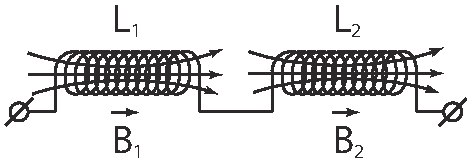
\includegraphics[width=.47\textwidth]{lec12/agreed_coils.pdf}
        \hfill
        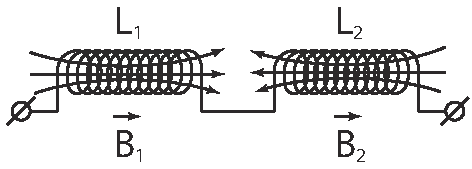
\includegraphics[width=.47\textwidth]{lec12/opposite_coils.pdf}
        \parbox[t]{.47\textwidth}{\caption{Согласованное соединение}}
        \hfill
        \parbox[t]{.47\textwidth}{\caption{Встречное соединение}}
    \end{figure}    

    \textbf{Согласованное соединение}
    Две последовательно соединённые соосные катушки включены
    \textit{согласованно}, если направление линий поля \( \vec{B} \) у одной
    катушки и у второй совпадают.
    
    \textbf{Встречное соединение}
    Две последовательно соединённые соосные катушки включены \textit{встречно},
    если направление линий поля \( \vec{B} \) у одной катушки противоположно
    направлениям линий поля у второй.
    
    Вычислим общую индуктивность \( L \) двух таких катушек. Пусть ток \( i \)
    -- общий. Тогда поток через \( N_1 \):
    \[
        \Phi_1 = L_1i \pm L_{21}i = (L_1 \pm M)i,
    \]
    где \( M \) -- взаимная индуктивность пары катушек, знак \( ``+'' \)
    ставится, если катушки подключены согласованно, \( ``-'' \) -- если
    встречно. Поток через \( N_2 \):
    \[
        \Phi_2 = L_2i \pm L_{12}i = (L_2 \pm M)i,
    \]
    а общий поток через две катушки:
    \[
        \Phi = \Phi_1 + \Phi_2 = (L_1 + L_2 \pm 2M)i.
    \]
    
    Тогда, по определению:
    \begin{equation}
        L = \frac{\Phi}{i} = L_1 + L_2 \pm 2M
    \end{equation}
    Если две катушки магнитно не связаны (\( M = 0 \)), то \( L = L_1 + L_2 \).
    Отсюда видно, что поворачивая катушки относительно друг друга можно плавно
    менять индуктивность на \( \Delta L = | 4M | \). Устройства с переменной
    индуктивностью называются \textit{вариометрами}.
    
    \subsection{Параллельное соединение}
    \begin{figure}[h]
        \center
        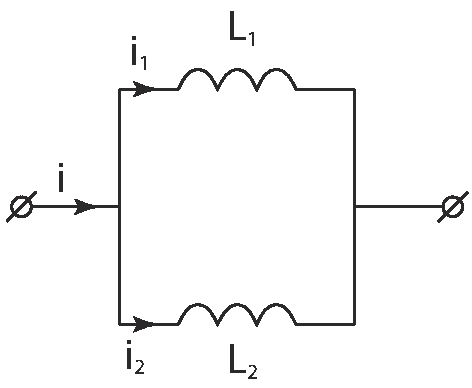
\includegraphics[width=0.3\textwidth]{lec12/parallel_coils.pdf}
    \end{figure}

    Вычислим индуктивность пары параллельно соединенных катушек, огранившись 
    случаем их магнитной несвязанности: \( M = 0 \). Видно, что \( i = i_1 + 
    i_2 \). При изменении тока:
    \begin{equation}
        \frac{\dd i}{\dd t} = \frac{\dd i_1}{\dd t} + \frac{\dd i_2}{\dd t}.
        \label{eq12:nn1}
    \end{equation}
    При этом в первой катушке наводится ЭДС:
    \[
        \EDS_1 = -L_1\frac{\dd  i_1}{\dd  t}.
    \]
    Аналогично, во второй катушке:
    \[
        \EDS_2 = -L_2\frac{\dd  i_2}{\dd  t}.
    \]
    Между точками \( a \) и \( b \):
    \[
        \EDS = -L\frac{\dd  i}{\dd  t},
    \]
    где \( L \) -- общая индуктивность. Тогда, с учетом (\ref{eq12:nn1}) и
    того, что \( \EDS_1 = \EDS_2 = \EDS \), получаем:
    \[
        \frac{\EDS_1}{L_1} + \frac{\EDS_2}{L_2} = \frac{\EDS}{L},
    \]
    или
    \begin{equation}
        \frac{1}{L_1} + \frac{1}{L_2} = \frac{1}{L}.
    \end{equation}
    
\section{Электрическое и магнитное давления}

    \begin{figure}[h]
        \center
        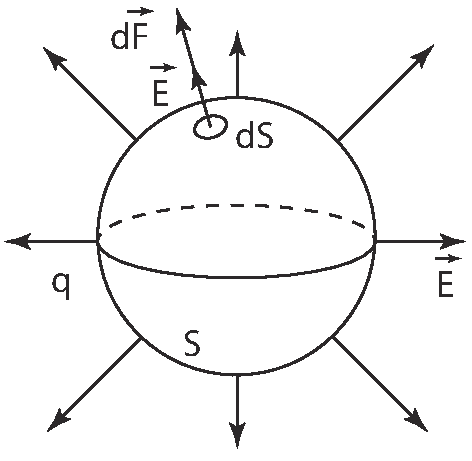
\includegraphics[width=.47\textwidth]{lec12/electric_pressure.pdf}
        \hfill
        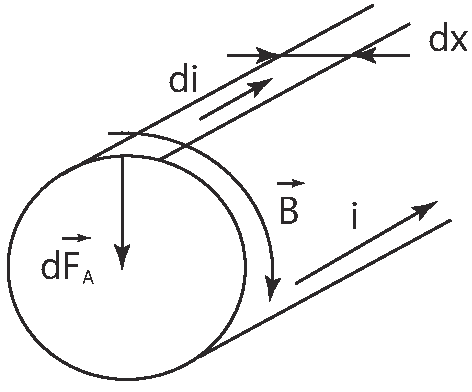
\includegraphics[width=.47\textwidth]{lec12/magnetic_pressure.pdf}
        \parbox[t]{.47\textwidth}{\caption{Давление электрического поля}}
        \hfill
        \parbox[t]{.47\textwidth}{\caption{Давление магнитного поля}}
    \end{figure}
\subsection{Давление электрического поля}

    Если в поле \( \vec{E} \) находится зарядовая поверхность, то поле оказывает
    на неё давление, причём оно направлено в сторону более сильного поля, то
    есть более сильное поле стремится сократить свой объем. Рассмотрим его
    механизм и вычислим его величину.
    
    Пусть зарядовая поверхность -- это поверхность металлического шара,
    содержащая заряд \( \sigma \). У поверхности металла
    \[
        E = \frac{\sigma}{\varepsilon_0}.
    \]
    Вырежем малый элемент поверхности \( \dd S \), несущий заряд
    \( \dd q = \sigma\dd S \).
    Тогда сверху:
    \[
        E = \frac{\sigma}{\varepsilon_0} = E_{\dd S} + E_{\textit{чуж}},
    \]
    где \( E_{\dd S} \) -- поле, создаваемое элементом \( \dd S \), а 
    \( E_{\textit{чуж}} \) -- поле, создаваемое всеми остальными элементами
    поверхности \( S \).
    
    Следовательно, элемент \( \dd S \) находится в чужом поле
    \[
        E_{\textit{чуж}} = \frac{\sigma}{\varepsilon_0} -
        \frac{\sigma}{2\varepsilon_0} = \frac{\sigma}{2\varepsilon_0}
    \]
    и на него действует сила
    \[
        \dd F = E_{\textit{чуж}}\dd q =
        \frac{\sigma}{2\varepsilon_0}\sigma\dd S =
        \frac{\sigma^2}{2\varepsilon_0}\dd S.
    \]
    Следовательно, давление:
    \[
        p_E = \frac{\dd F}{\dd S} = \frac{\sigma^2}{2\varepsilon_0} = 
        \frac{\varepsilon_0^2E^2}{2\varepsilon_0}.
    \]
    
    Таким образом, давление электрического поля:
    \begin{equation}
        p_E = \frac{\varepsilon_0E^2}{2}.
    \end{equation}
    
    \begin{remark}
        Внизу площадки \( \dd S \) поле \( E_{\textit{рез}} = E_{\dd S} - 
        E_{\textit{чуж}} = 0 \), поэтому внутри проводника поля нет.
    \end{remark}

    \begin{example}
        Пусть сфера радиуса \( R = 0,1 \)м заряжена до потенциала
        \( \varphi = 1 \) МВ. Определить давление поля \( \vec{E} \) на сферу.
    \end{example}
    
    \begin{solution}
        Внутри сферы поле \( E = 0 \), а вне её
        \[
            E = \frac{\varphi}{R},
        \]
        Таким образом, поле \( E = \frac{10^6}{10^{-1}} = 
        10^7 \text{В}/\text{м} \).
        Тогда давление:
        \[
            p_E = \frac{\varepsilon_0 E^2}{2} = \frac{10^{-11} \cdot 10^{14}}{2}
            = 500 \text{Па} = 5 \times 10^{-3} \text{атм}
        \]
    \end{solution}
    
    \begin{remark}
        Если с одной стороны от зарядовой поверхности поле \( E = E_1 \), а с
        другой -- поле \( E = E_2 \), то давление \( p_E \):
        \begin{equation}
            p_E = \frac{\varepsilon_0}{2}|E_1^2 - E_2^2|
        \end{equation}
        Оно направлено в сторону более сильного поля.
    \end{remark}

\subsection{Давление магнитного поля}
    Магнитное поле оказывает давление на токовые поверхности, стремясь увеличить
    свой объем. Токовой поверхностью может быть, например, стенка соленоида. В 
    основе механизма давления магнитного поля лежит действие силы Ампера на
    токовые поверхности. Рассмотрим трубку радиуса \( R \) с током \( i \).
    
    Сила Ампера, действующая на полоску (\( l, \dd x \)):
    \[
        \dd \vec{F}_A = \dd i(\vec{l}\times\vec{B}_{\textit{чуж}}),
    \]
    где \( \dd i = j\dd x \) -- ток полоски, \( \dd x \) -- ширина полоски,
    \( B_{\textit{чуж}} \) -- поле, созданное остальными элементами трубки,
    \( j = \frac{i}{2\pi R}\text{А}/\text{м} \) -- поверхностная плотность тока.
    \[
        \dd \vec{F}_A = j\dd x\vec{l}\times\vec{B}_{\textit{чуж}} =
        j\dd \vec{S}\times\vec{B}_{\textit{чуж}}.
    \]
    Поле у поверхности трубки
    \[
        B = B_{\dd x} + B_{\textit{чуж}} = \frac{\mu_0i}{2\pi R} = \mu_0j.
    \]
    А так как поле у поверхности поолоски
    \[ 
        B_{\dd x} = \mu_0\frac{j}{2},
    \]
    то
    \[
        B_{\textit{чуж}} = B - B_{\dd x} = \mu_0j - \mu_0\frac{j}{2} =
        \mu_0\frac{j}{2}.
    \]
    \[
        \dd \vec{F}_A = j\dd S\mu_0\frac{j}{2} = \frac{\mu_0j^2}{2}\dd S =
        \frac{B^2}{2\mu_0}\dd S.
    \]
    
    Таким образом, давление магнитного поля:
    \begin{equation}
        p_B = \frac{\dd \vec{F}_A}{\dd S} = \frac{B^2}{2\mu_0}.
        \label{eq12:LetItBeTheLabel}
    \end{equation}
    
    \begin{remark}
        Если с одной стороны от токовой поверхности поле \( B = B_1 \),
        а с другой -- поле \( B = B_2 \), то давление магнитного поля:
        \begin{equation}
            p_B = \frac{1}{2\mu_0}|B_1^2 - B_2^2|
        \end{equation}
        Оно направлено в сторону более слабого поля.
    \end{remark}
    
    \begin{example}
        Пусть в соленоиде поле \( B = 1 \)Тл. Определить давление поля на стенки
        соленоида.
    \end{example}
    
    \begin{solution}
        По формуле (\ref{eq12:LetItBeTheLabel})
        \[
            p_B = \frac{B^2}{2\mu_0} = \frac{1}{2\times10^{-6}} = 500 \text{кПа}
            = 5 \text{атм}
        \]
    \end{solution}
    
    \begin{example}
        По трубке радиуса \( R = 0,01 \)м прошёл разряд молнии током
        \( i = 300 \)кА и смял её. Определить давление поля \( B \).
    \end{example}
    
    \begin{solution}
        Поле
        \[
            B = \frac{\mu_0i}{2\pi R} = 
            \frac{10^{-6}\cdot3\times10^5}{6\times10^{-2}} = 5\text{Тл}.
        \]
        
        Тогда давление поля
        \[
            p_B = \frac{B^2}{2\mu_0} = \frac{25}{2\times10^{-6}} =
            10^7 \text{Па} = 100 \text{атм} 
        \]
    \end{solution}
